% Indicate the main file. Must go at the beginning of the file.
% !TEX root = ../main.tex

%----------------------------------------------------------------------------------------
% CHAPTER TEMPLATE
%----------------------------------------------------------------------------------------


\chapter{Experimentació} % Main chapter title

\label{Experimentació} % Change X to a consecutive number; for referencing this chapter elsewhere, use \ref{ChapterX}
En aquest apartat s'expliquen en detall els criteris seguits per generar les instàncies, com aquesta afecten la seva complexitat i temps de resolució, com s'han obtingut i recollit tots els resultats, juntament amb la comparativa del rendiment de cada millora que ha rebut el model.

\section{Generació d'instàncies}
La generació d'instàncies s'ha fet mitjançat la pàgina web desenvolupada \ref{subsec:generar-instancies}, la qual ha ajudat molt a poder captar visualment les implicacions que impliquen els inputs del model a la complexitat de les instàncies.\\
A banda un cop generades i guardades les instàncies en fitxer .json, s'ha fet ús d'un script en Python \ref{AppendixB} que itera per tots els fitxers i guarda les dades més importants en un fitxer excel per més tard poder analitzar de forma més fàcil les característiques de cada instància.
Tot i que la generació en si ha sigut còmode de fer, hi ha hagut un raonament darrere a l'hora de decidir quins havien de ser els inputs:

\subsection{Mida del blueprint}
Aquest input és un dels que més afecta la complexitat de la instància, ja que la majoria de variables del model augmenten exponencialment en funció d'aquest input, per això s'ha decidit crear instàncies amb mides que van des de 5x5 fins a 8x8, ja que 5x5 és la mida mínima on es pot encabir un assemblador i les seves entrades i 8x8 és la mida màxima on el model pot trobar solucions en un temps raonable. Per cada rang de mides s'han generat múltiples instàncies jugant amb altres paràmetres d'entrada.

\subsection{Objecte a produir}
L'objecte a produir al blueprint és una de les entrades del model més interessants, ja que implica moltes coses. Primer un objecte determinat pot implicar una o més receptes, aquestes receptes requereixen un assemblador i a més poder requerir certs objectes d'entrada en diferents quantitats. A causa de la gran quantitat de factors que s'han de tenir en compte a l'hora de triar l'objecte a produir s'ha decidit separar en quantitat de receptes associades a l'objecte a produir i la quantitat d'objectes d'entrada requerits. Així doncs s'han creat instàncies amb el mateix nombre de receptes associades i diferent quantitat d'objectes d'entrada, a més també hi ha instàncies amb el mateix nombre de receptes i objectes d'entrada on es juga amb les ràtios dels objectes d'entrada respecte a la quantitat d'objectes produïts.\\

\subsection{Posicions d'entrada i sortida}
Finalment per afegir diversitat a les instàncies per una mateixa configuració d'objecte a produir i mida, s'han escollit diferents maneres de fer entrar i sortir els objectes per veure com afecta la solució de la instància.

\section{Instàncies generades}
Les instàncies creades amb els anteriors criteris han sigut 41. Per poder veure més en detall com és cada instància, s'ha creat una taula on per cada instància es mostren les mètriques més importants, mida, receptes implicades, objectes implicats, objectes d'entrada únics, nombre d'entrades i nombre de sortides. Aquesta taula és molt útil per més endavant veure la relació entre les mètriques d'entrada i les seves implicacions al temps de resolució i complexitat.\\
Concretament per cada instància es mostren els valors descrits al capítol \ref{disseny model} on les taules \ref{route-variables}, \ref{assembler-variables}, \ref{item_flow-variables}, \ref{item_flow_rate-variables} i \ref{recipe-variables}. Aquestes mostren les variables usades per les restriccions i les seves mides i dominis en funció l'input de la instància, els valors dels quals apareixen a les següents taules. Amb aquesta representació es pot veure el pes de cada instància sobre les variables anteriorment descrites.

\begin{figure}[H]
    \centering
    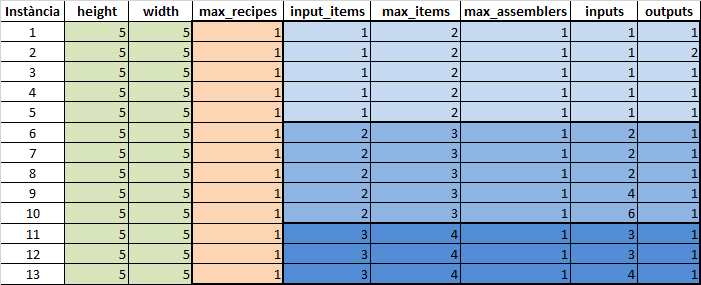
\includegraphics[width=1\linewidth]{Figures/miscelaneous/instances_5x5.png}
    \caption{Instàncies amb mida 5x5}
\end{figure}
\begin{figure}[H]
    \centering
    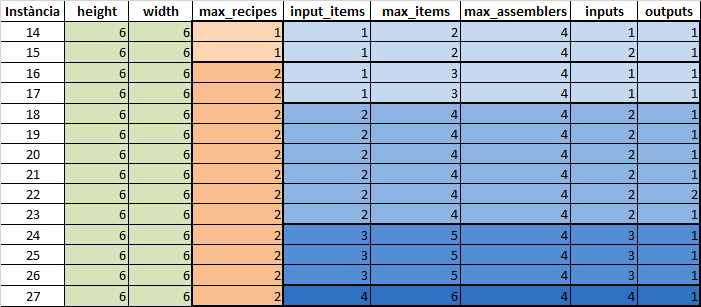
\includegraphics[width=1\linewidth]{Figures/miscelaneous/instances_6x6.png}
    \caption{Instàncies amb mida 6x6}
\end{figure}
\begin{figure}[H]
    \centering
    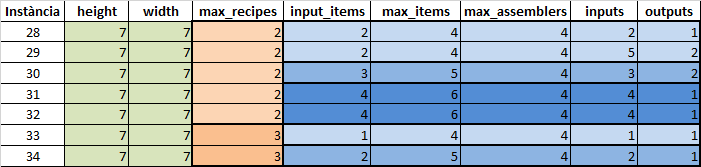
\includegraphics[width=1\linewidth]{Figures/miscelaneous/instances_7x7.png}
    \caption{Instàncies amb mida 7x7}
\end{figure}
\begin{figure}[H]
    \centering
    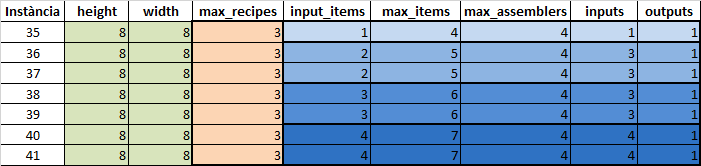
\includegraphics[width=1\linewidth]{Figures/miscelaneous/instances_8x8.png}
    \caption{Instàncies amb mida 8x8}
\end{figure}

\section{Models de proves}
Les múltiples millores que el model base ha rebut al llarg del projecte ha donat lloc a cinc versions. Aquestes s'han posat a prova resolent les instàncies anteriorment descrites, amb els tres criteris d'optimització implementats (maximització de l'objecte a fabricar, minimització de les rutes i minimització de la pèrdua d'objectes).\\
Les diferents versions del model són les següents:

\subsection{Primera versió (model base)}
Aquest model tracta de la base on s'han anat aplicant les millores i el que ha sigut descrit durant l'apartat \ref{model-base} juntament amb els canvis relacionats a les mecàniques del joc explicades a la secció \ref{mecanics-changes}. El seu rendiment és molt pobre respecte els models subseqüents, però s'ha avaluat amb la resta per poder veure la progressió que s'ha seguit al llarg del projecte.

\subsection{Segona versió (pre càlcul i bounds)}
La segona versió és la que conté les millores que més han afectat al rendiment, concretament incorpora el pre càlcul de les receptes \ref{precompute-recipes}, el lower bound respecte al nombre d'assembladors presents al blueprint \ref{lower-bound} i l'upper bound referent al domini de la variable \texttt{route} \ref{upper-bound}

\subsection{Tercera versió (trencament de simetries 1)}
Les millores aplicades en aquest model són les del model anterior juntament amb el trencament de les simetries explicat a la secció \ref{mecanics-changes}. Tot i que a la secció mencionada només s'explica la versió final del trencament de simetries aquesta té una versió anterior molt similar que no ordena la variable auxiliar \texttt{used}, tot i que el canvi en codi és mínim s'ha considerat usar les dues versions als experiments per veure si el canvi és gaire notori.

\subsection{Quarta versió (trencament de simetries 2)}
Aquesta versió conté el trencament de simetries amb la petita millora de l'ordenació de la variable \texttt{used} a la implementació del trencament de la simetria.

\subsection{Cinquena versió (inseridors redundants)}
L'última versió del model incorpora l'optimització més important després del pre-calcul i els bounds, aquesta tracta de l'eliminació de la possibilitat d'usar inseridors en posicions on són redundants, afegint moltes solucions "simètriques" \ref{prevent-redundant-inserters}.

\section{Resultats}
Per posar a prova tots els models s'han resolt les quaranta-una instàncies usant els tres criteris d'optimització amb un time-out de trenta minuts. Les solucions a les instàncies, com s'ha explicat anteriorment, s'han descarregat i amb l'ajuda d'un script en Python \ref{AppendixC} s'han posat en comú tots els resultats en un fitxer Excel on s'han pogut generar tots els gràfics.\\
Els resultats s'han dividit en tres parts:
\subsection{Nombre d'instàncies resoltes}\label{subsec:instances-solved}
En aquesta secció es fa una comparativa entre les 5 versions del model i la quantitat d'instàncies que han pogut resoldre respecte a les que no s'han pogut resoldre en menys de trenta minuts. A més també es comparen aquests resultats per cada criteri d'optimització.

\begin{figure}[H]
    \centering
    \begin{subfigure}{0.4\textwidth}
        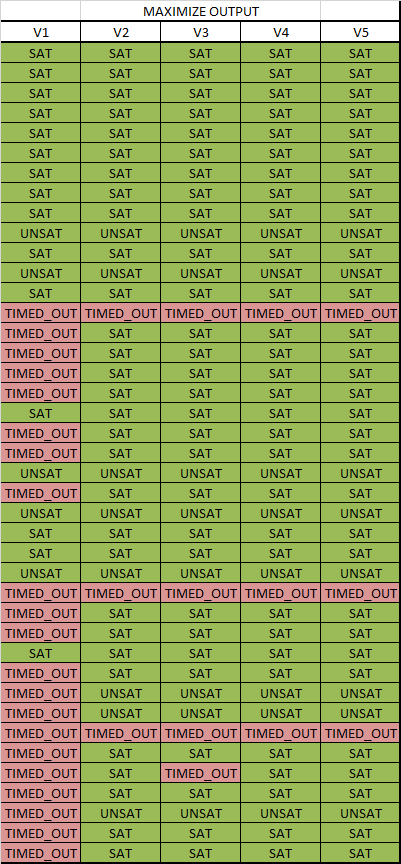
\includegraphics[width=\textwidth]{Figures/experiment_results/instances_solved_1.png}
    \end{subfigure}
    \hfill
    \begin{subfigure}{0.4\textwidth}
        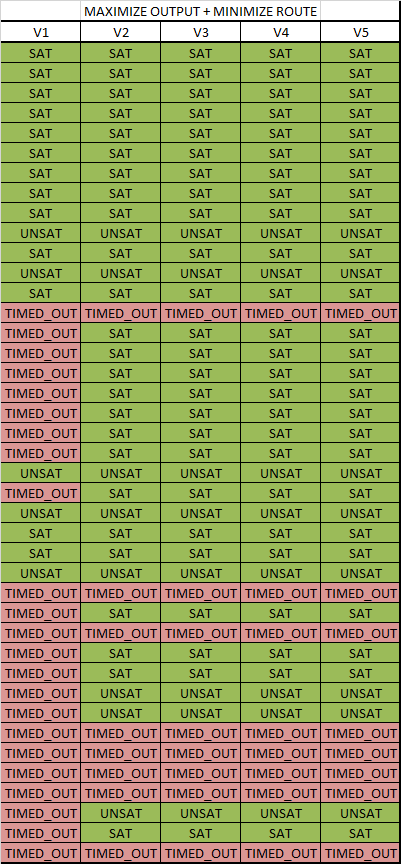
\includegraphics[width=\textwidth]{Figures/experiment_results/instances_solved_2.png}
    \end{subfigure}
    \hfill
    \begin{subfigure}{0.4\textwidth}
        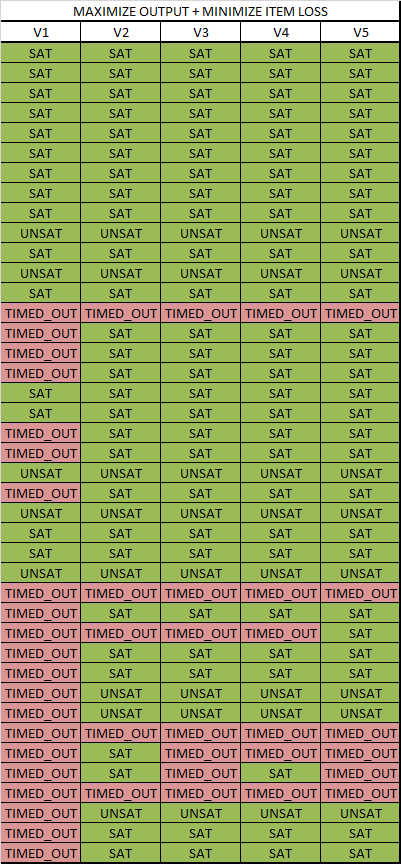
\includegraphics[width=\textwidth]{Figures/experiment_results/instances_solved_3.png}
    \end{subfigure}
    \caption{Resultat de cada instància per cada versió del model i cada criteri d'optimització}
\end{figure}

Amb aquestes taules es pot veure com la millora més dràstica és entre la primera i la segona versió del model, que és on hi ha hagut la majora de canvis importants, entre les altres versions, els canvis són mínims i en alguns casos fins i tot hi ha alguna instància que no es resol en una versió del model posterior que anteriorment si havia sigut resolta.\\
Tot seguit un recompte de les instàncies resoltes per poder veure millor el rendiment entre versions:

\begin{figure}[H]
    \centering
    \begin{subfigure}{0.6\textwidth}
        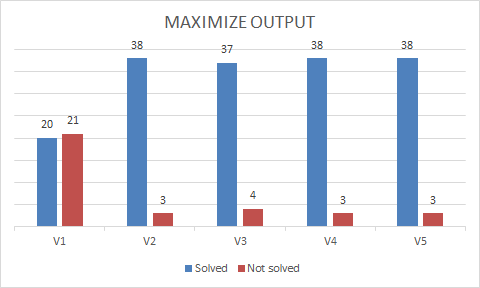
\includegraphics[width=\textwidth]{Figures/experiment_results/solved_instances_count_1.png}
    \end{subfigure}
    \hfill
    \begin{subfigure}{0.6\textwidth}
        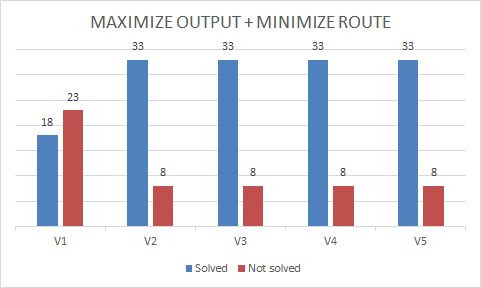
\includegraphics[width=\textwidth]{Figures/experiment_results/solved_instances_count_2.png}
    \end{subfigure}
    \hfill
    \begin{subfigure}{0.6\textwidth}
        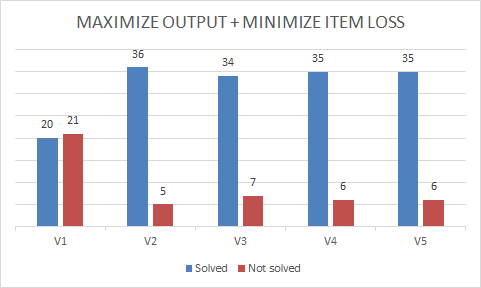
\includegraphics[width=\textwidth]{Figures/experiment_results/solved_instances_count_3.png}
    \end{subfigure}
    \caption{Nombre d'instàncies resoltes i no resoltes per versió i optimització}
\end{figure}

Amb els diagrames de barres es pot apreciar encara més el canvi entre la primera versió i les posteriors, a més també es veu com amb el criteri d'optimització que minimitza la mida de la ruta s'aconsegueixen resoldre forces menys instàncies respecte al criteri d'optimització que minimitza la pèrdua d'objectes.\\

Un detall important a mencionar és que hi ha certes instàncies que no es poden resoldre en cap de les versions, aquestes instàncies tracten concretament de la 14, 28 i 35, les quals per la mida del blueprint que tenen, el nombre de receptes que s'utilitzen i com a conseqüència el nombre d'assembladors que s'usaran és molt inferior al nombre màxim d'assembladors que hi entren. Aquesta diferència fa que el solver tingui moltes més opcions vàlides a l'hora de disposar els assembladors que es necessitaran, fent que el temps de resolució es dispari. Per aquest motiu s'ha jugat amb el nombre d'entrades del blueprint, per poder ajudar al solver reduït el nombre de possibles assignacions vàlides i reduint l'espai de solucions.

\subsection{Temps de resolució}
A continuació es mostra el temps que s'ha necessitat per resoldre cada instància per cada versió del model i criteri d'optimització juntament amb la comparació entre els temps de resolcuó de cada versió del model.

\begin{figure}[H]
    \centering
    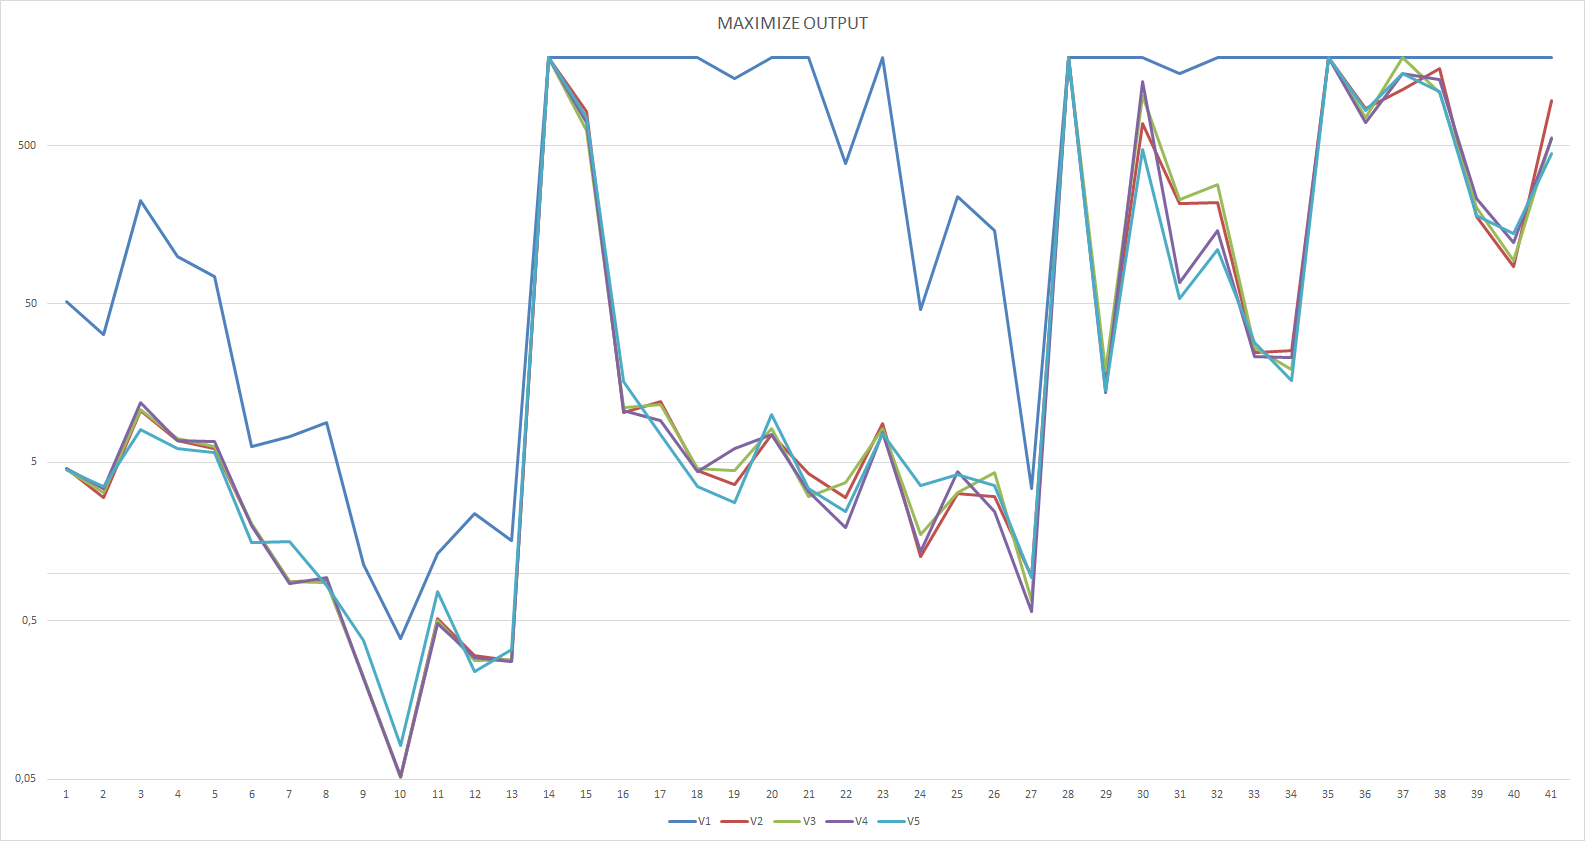
\includegraphics[width=1\linewidth]{Figures/experiment_results/solving_time_1.png}
    \caption{Comparació entre els temps de resolució dels cinc models amb el criteri d'optimització de maximitzar l'objecte objectiu}
    \label{fig:opt1_times}
\end{figure}

\begin{figure}[H]
    \centering
    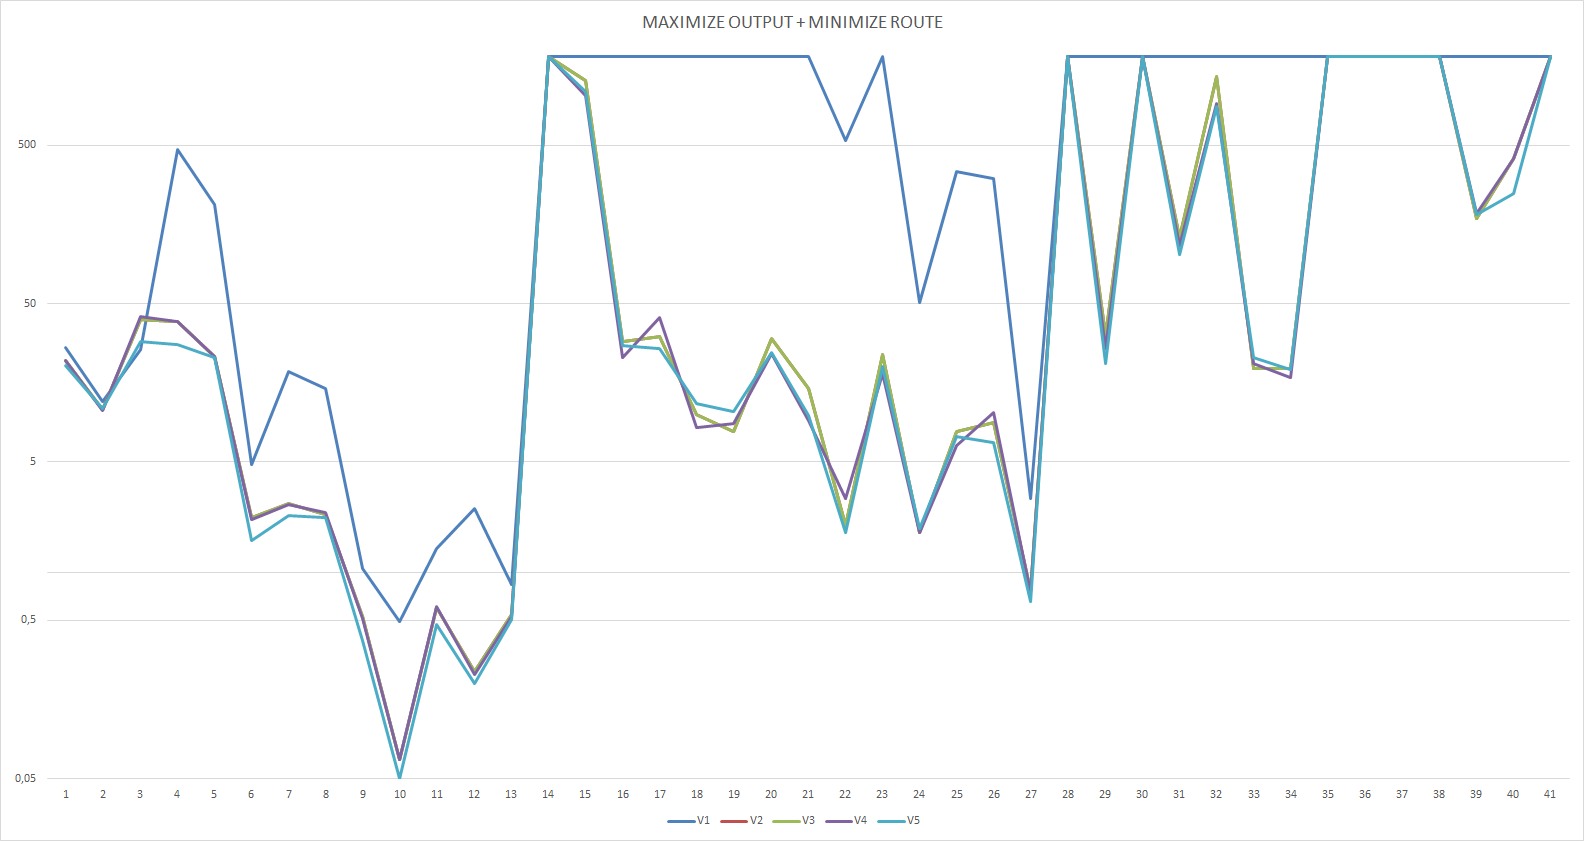
\includegraphics[width=1\linewidth]{Figures/experiment_results/solving_time_2.png}
    \caption{Comparació entre els temps de resolució dels cinc models amb el criteri d'optimització de minimitzar la mida de les rutes}
    \label{fig:opt2_times}
\end{figure}

\begin{figure}[H]
    \centering
    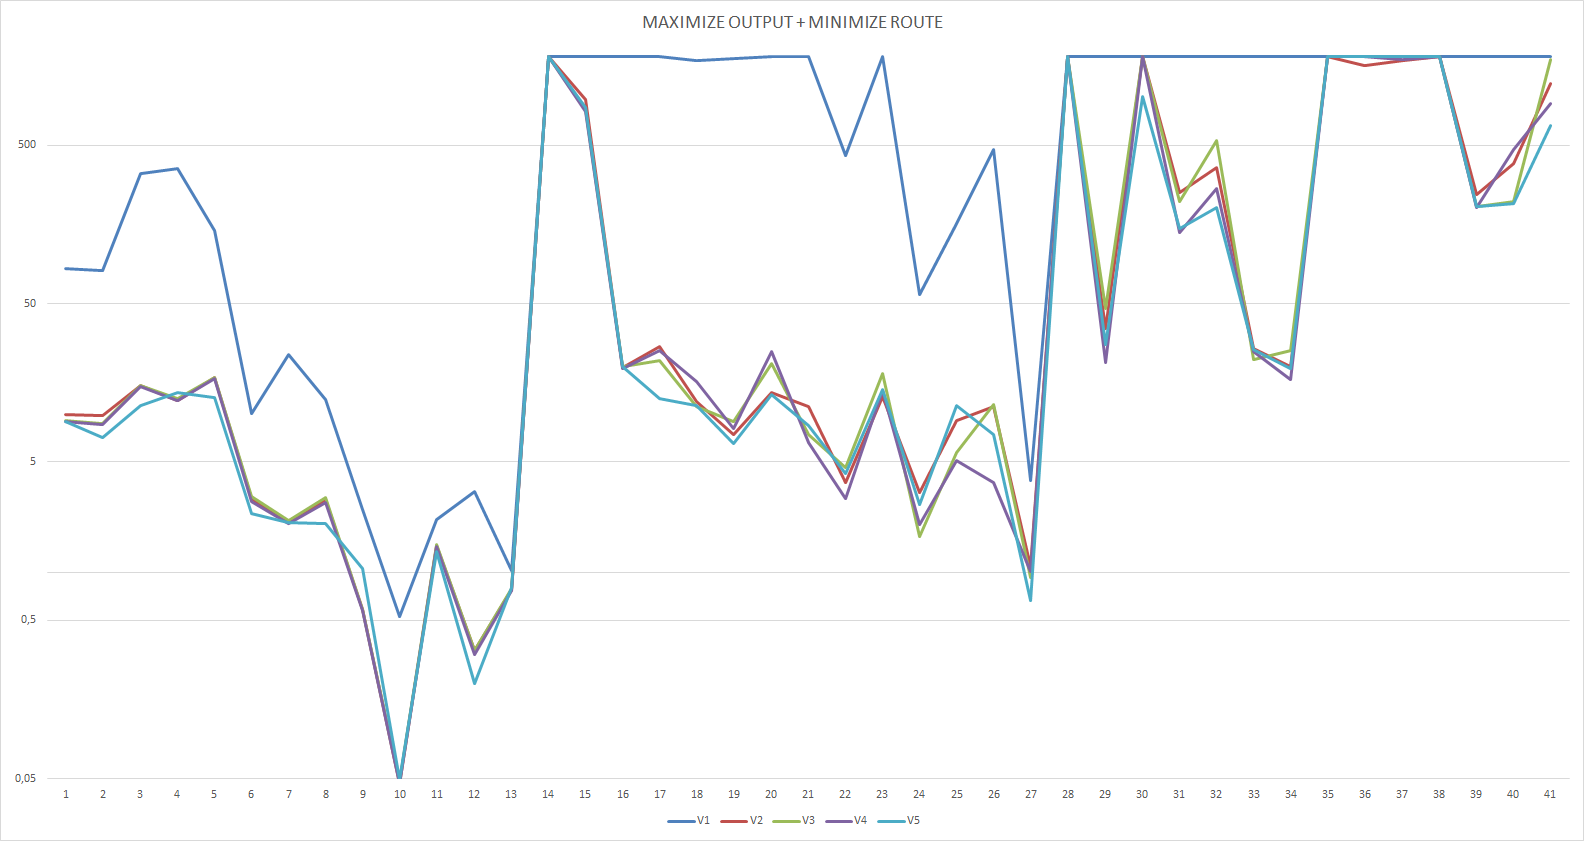
\includegraphics[width=1\linewidth]{Figures/experiment_results/solving_time_3.png}
    \caption{Comparació entre els temps de resolució dels cinc models amb el criteri d'optimització de minimitzar la pèrdua d'objectes}
    \label{fig:opt3_times}
\end{figure}

Els diagrames anteriors s'han representat en escala logarítmica a causa de la gran diferència de temps algunes d'elles, d'aquesta manera és més fàcil apreciar visualment les diferències entre les versions.\\

Si analitzem els diagrames, es poden diferenciar els quatre grups d'instàncies de mides 5x5, 6x6, 7x7 i 8x8. Ja que com s'ha explicat la mida del blueprint és un dels inputs que més repercussió té a la complexitat de la instància. Aquesta diferència es manté per tots els criteris d'optimització.\\
A banda es pot veure com al llarg de les instàncies hi ha pics i valls molt notoris, els pics són deguts principalment a les instàncies que són particularment difícils pel motiu comentat a la secció \ref{subsec:instances-solved}. Les valls d'altra banda són degudes a les instàncies que no tenen una solució satisfacible, aquestes instàncies ha resultat ser més senzilles segurament degut al fet que l'espai proporcionat envers la quantitat d'assembladors necessaris és massa poc fet sembla ajudar a propagar molt al solver fent que la solució es trobi més abans.\\




\subsection{Representació gràfica d'algunes instàncies resoltes}



